\begin{figure}[htbp]
			\centering
			\begin{tikzpicture}[scale=0.95,>=latex,
				trave/.style={line width=1.2pt},
				carico/.style={black, line width=0.5pt},
				diagN/.style={black, line width=0.8pt},
				hatch/.style={gray!40, line width=0.3pt},
				puntotang/.style={circle, fill=black, inner sep=1.1pt},
				]
				% ── Parametri ──
				\def\tw{0.15}\def\thR{0.28}\def\rn{0.06}
				\def\rw{0.05}\def\bw{0.09}\def\gw{0.22}\def\hh{0.10}
				\def\Lb{4}\def\hq{0.8}\def\bb{0.10}\def\fa{0.13}
				\def\hN{0.45}     % scala del diagramma N0 (qbar*l/pi -> hN)
				% ── Vincoli ──
				\def\cerniera#1{%
					\draw[thick] (#1,0) -- (#1-\tw,-\thR) -- (#1+\tw,-\thR) -- cycle;
					\draw[thick] (#1-\gw,-\thR) -- (#1+\gw,-\thR);
					\foreach \x in {-0.16,-0.08,0,0.08,0.16}
					\draw[thin] (#1+\x,-\thR) -- ++(-0.07,-\hh);
					\draw[thick, fill=white] (#1,0) circle (\rn);}
				\def\carrello#1{%
					\draw[thick] (#1,0) -- (#1-\tw,-\thR) -- (#1+\tw,-\thR) -- cycle;
					\draw[thick] (#1-\bw,-\thR-\rw-0.01) circle (\rw);
					\draw[thick] (#1+\bw,-\thR-\rw-0.01) circle (\rw);
					\draw[thick] (#1-\gw,-\thR-2*\rw-0.04) -- (#1+\gw,-\thR-2*\rw-0.04);
					\foreach \x in {-0.16,-0.08,0,0.08,0.16}
					\draw[thin] (#1+\x,-\thR-2*\rw-0.04) -- ++(-0.07,-\hh);
					\draw[thick, fill=white] (#1,0) circle (\rn);}
				% ── Carico armonico longitudinale ──
				\def\caricoarmonico{%
					\draw[carico] plot[domain=0:\Lb, samples=90] (\x, {\bb + \hq*sin(45*\x)});
					\draw[carico] (0,\bb) -- (\Lb,\bb);
					\foreach \s in {0.5,1.0,1.5,2.0,2.5,3.0,3.5}
					\draw[carico] (\s,\bb) -- (\s, {\bb+\hq*sin(45*\s)});
					\foreach \s in {0.5,1.0,1.5,2.0,2.5,3.0,3.5}
					\draw[->, carico] (\s,{\bb+\fa}) -- (\s+0.32,{\bb+\fa});
					\node[font=\small] at (2.95,{\bb+\hq+0.16}) {$\bar{q}$};
					\draw[carico, ->] (2.78,{\bb+\hq+0.10}) -- (2.0,{\bb+\hq/2});
				}
				
				% ===================== (a) sistema principale, solo carico =====================
				\begin{scope}[xshift=0cm]
					\draw[trave] (0,0) -- (\Lb,0);
					\cerniera{0}\carrello{\Lb}
					\node[above left=-2pt, font=\small] at (0,0) {$A$};
					\node[above=1pt, font=\small] at (\Lb,0.05) {$B$};
					\caricoarmonico
					\node[font=\small] at (\Lb/2,-0.75) {(a)};
				\end{scope}
				
				% ===================== (b) diagramma N0 (trazione, sopra l'asse) =====================
				\begin{scope}[xshift=6.2cm]
					\draw[trave] (0,0) -- (\Lb,0);
					% campitura
					\foreach \x in {0.1,0.3,...,3.9}
					\draw[hatch] (\x,0) -- (\x, {\hN*(1+cos(45*\x))});
					% contorno: chiusura verticale in A + curva 1+cos
					\draw[diagN] (0,0) -- (0,{2*\hN})
					plot[domain=0:\Lb, samples=100] (\x, {\hN*(1+cos(45*\x))});
					% flesso in mezzeria
					\node[puntotang] at (2,\hN) {};
					\cerniera{0}\carrello{\Lb}
					\node[above left=-2pt, font=\small] at (0,0) {$A$};
					\node[above right=-2pt, font=\small] at (\Lb,0) {$B$};
					\node[font=\small] at (1.0,0.42) {$\boldsymbol{\oplus}$};
					\node[left=-2pt, font=\small] at (0,{2*\hN}) {$\tfrac{2\bar{q}\ell}{\pi}$};
					\node[above, font=\scriptsize] at (2,\hN) {$\tfrac{\bar{q}\ell}{\pi}$};
					%\node[font=\small] at (2.9,0.55) {$N_0$};
					\node[font=\small] at (\Lb/2,-0.75) {(b)};
				\end{scope}
				
			\end{tikzpicture}
			\caption{(a)~problema ``0'': sistema principale soggetto al solo carico;
				(b)~sforzo normale $N_0$, in trazione, decrescente da $2\bar{q}\ell/\pi$
				in $A$ a zero in $B$, con flesso in mezzeria.}
			\label{fig:stat_iper_long_01-p0}
		\end{figure}
